% In this section, we start with a review of the prior work of adaptive data analysis, which motivates our work, a framework to statically give an upper bound on the rounds of adaptivity . We then show the architecture of the framework and give our readers a taste from simple examples. 

% \subsection{Review of Prior Work}

% To explain the key concepts and motivate our work, we review the model of adaptive data analysis of~\cite{DworkFHPRR15,HU14}.  We remark that many of the details of the model are immaterial for our work, and are included for illustrative purposes and concreteness.  

\paragraph{Some results in Adaptive Data Analysis}
In Adaptive Data Analysis an \emph{analyst} is interested in studying some distribution $\dist$ over some domain $\univ$.  Following previous works~\cite{DworkFHPRR15,HardtU14,BassilyNSSSU16}, we focus on the setting where the analyst is interested in answers to \emph{statistical queries} (also known as \emph{linear queries}) over the distribution.  A statistical query is usually defined by some function $\query \from \univ \to [-1,1]$ (often other codomains such as $[0,1]$ or $[-R,+R]$, for some $R$, are considered).  The analyst wants to learn the \emph{population mean}, which (abusing notation) is defined as $$\query(\dist) = \ex{\sample \sim \dist}{\query(\sample)}.$$

However, the distribution $\dist$ can only be accessed via a set of \emph{samples} $\sample_1,\dots,\sample_n$ drawn from $\dist$. We assume that the samples are drawn independently and identically distributed (i.i.d.).  These samples are held by a mechanism $\mech(\sample_1,\dots,\sample_n)$ who receives the query $\query$ and computes an answer 
$$\answer \approx \query(\dist).$$

The na\"ive way to approximate the population mean is to use the \emph{empirical mean}, which (abusing notation) is defined as $$\query(\sample_1,\dots,\sample_n) = \frac{1}{n} \sum_{i=1}^{n} \query(X_i).$$
However, the mechanism $M$ can then adopt some methods for improving the generalization error.

In this work we consider analysts that ask a sequence of $k$ queries $\query_1,\dots,\query_k$.  If the queries are all chosen in advance, independently of the answers of each one of them, then we say they are \emph{non-adaptive}.  If the choice of each query $\query_j$ depend on the prefix $\query_1,\answer_1,\dots,\query_{j-1},\answer_{j-1}$ then they are \emph{fully adaptive}.  An important intermediate notion is \emph{$\qrounds$-round adaptive}, where the sequence can be partitioned into $\qrounds$ batches of non-adaptive queries.  Note that non-interactive queries are $1$-round and fully adaptive queries are $k$ rounds.

We now review what is known about the problem of answering $r$-round adaptive queries.  
\begin{thm} 
\label{thm:nonadapt-adapt}
For any distribution $\dist$, and any $k$ \emph{non-adaptive} statistical queries, the empirical mean satisfies
$$
\max_{j=1,\dots,k} | \answer_j - \query_j(\dist) | = O\left( \sqrt{\frac{\log k}{n}}  \right)
$$
For any $\qrounds \geq 2$ and any \emph{$\qrounds$-round adaptive} statistical queries, it satisfies
$$
\max_{j=1,\dots,k} | \answer_j - \query_j(\dist) | = O\left( \sqrt{\frac{k}{n}}  \right)
$$
\end{thm}
In fact, these bounds are tight (up to constant factors) which means that even allowing one extra round of adaptivity leads to an exponential increase in the generalization error of the empirical mean, from $\log k$ to $k$.

\citet{DworkFHPRR15} and \citet{BassilyNSSSU16} showed that by using an alternative mechanism $M$ which uses randomization in order to limit the dependency of a single query on the specific data instance, one 
can actually achieve much stronger generalization error as a function of the number of queries, specifically.
\begin{thm}[\cite{DworkFHPRR15, BassilyNSSSU16}] \label{thm:gaussiannoise} For any $k$, there exists a mechanism such that for any distribution $\dist$, and any $\qrounds \geq 2$ any \emph{$\qrounds$-round adaptive} statistical queries, it satisfies
$$
\max_{j=1,\dots,k} | \answer_j - \query_j(\dist) | = O\left( \frac{\sqrt[4]{k}}{\sqrt{n}}  \right)
$$
%And there is an analyst that make this bound tight (up to constant factors).
\end{thm}
Notice that Theorem~\ref{thm:gaussiannoise} has different quantification in that the optimal choice of mechanism depends on the number of queries.  Thus, we need to know the number of queries \emph{a priori} to choose the best mechanism.
% \footnote{ \label{fn1} One can, in principle, avoid knowing the number of queries and rounds \emph{a priori} using a ``guess-and-double'' strategy, however this would weaken the bound on generalization error considerably.}


%Later work by Dwork 
% \etal~\cite{??} 
\citet{DworkFHPRR15}
also gave more refined bounds in terms of the number of rounds of adaptivity.   %\footnotemark[\ref{fn1}] 
%Specifically, 
\begin{thm}[\cite{DworkFHPRR15}] \label{thm:gaussiannoise2} For any $r$ and $k$, there exists a mechanism such that for any distribution $\dist$, and any $\qrounds \geq 2$ any \emph{$\qrounds$-round adaptive} statistical queries, it satisfies
$$
\max_{j=1,\dots,k} | \answer_j - \query_j(\dist) | = O\left( \frac{r \sqrt{\log k}}{\sqrt{n}}  \right)
$$
%And there is an analyst that make this bound tight (up to constant factors).
\end{thm}

This suggests that if one knows a good \emph{a priori upper bound on the number of rounds of adaptivity}, one can get a much better guarantee of generalization error, but only by using an appropriate choice of the mechanism.

\wq{Let us have a look at an example to better understand the impact of adaptivity in the choice of mechanism to control the generalization error.  }
\jl{
In Figure~\ref{fig:generalization_errors}, the x axis is Queries in this Data analysis sent to Server in each step of the data analysis,
The y axis is Generalization Error of analysis result computed from every query.
\\
In Figure~\ref{fig:generalization_errors}(a) where the data analysis
has $k = 500$ non-adaptive queries but only $r = 2$ rounds 
of adaptivity.
By choosing different mechanisms, the generalization error is reduced in different degree.
It is obvious than we got better generalization results by choosing the data splitting mechanism than Gaussian mechanism.
\\
However, in figure~\ref{fig:generalization_errors}(b), where the data analysis 
has $k = 500$ queries in total as well as $r= 500$ rounds of adaptivity.
\\
The generalization error is increasing as the query increasing, i.e., as the adaptivity 
accumulating.
In this $500$ rounds adaptive data analysis, by choosing Gaussian mechanism, we got better generalization results than choosing the data splitting mechanism.
}
{\small
\begin{figure}
\centering
\begin{subfigure}{.48\textwidth}
\begin{centering}
\includegraphics[width=0.9\textwidth]{tworound.png}
\caption{}
\end{centering}
\end{subfigure}
%}
% \quad
% \centering
% \begin{subfigure}{.3\textwidth}
% \begin{centering}
% \includegraphics[width=0.9\textwidth]{tworound_datasplitting.png}
% \caption{}
% \end{centering}
% \end{subfigure}
%}
\quad
\begin{subfigure}{.48\textwidth}
\begin{centering}
\includegraphics[width=0.9\textwidth]{multipleround.png}
\caption{}
\end{centering}
\end{subfigure}
\vspace{-0.4cm}
 \caption{
 The generalization errors of two adaptive data analysis examples, under different choices of mechanisms.
 (a) Data analysis with adaptivity 2, 
 (b) Data analysis with adaptivity 500. 
}
\label{fig:generalization_errors}
\vspace{-0.5cm}
\end{figure}
}

\paragraph{{A formal model for adaptivity}}
Motivated by the results discussed above, we will present a static analysis aimed at giving good \emph{a priori} upper bounds on the number of rounds of adaptivity of a program. Before introducing the static analysis, we motivate the definition of adaptivity we will use through a simple example illustrated in Figure~\ref{fig:overview-example}(a), which implements a simple "two rounds strategy" in our query while language presented in Section~\ref{sec:loop_language}.

{\small
\begin{figure}
\centering
\begin{subfigure}{.25\textwidth}
\begin{centering}
% $
% \begin{array}{l}
%   a \leftarrow 0; \\
%   i \leftarrow 0 ; \\
%     \eloop ~ 3 ~ \edo ~ \\
%     \quad
%      x \leftarrow q_1(\chi[i])   ; \\
%     \quad a \leftarrow a+x; \\
%         \quad i \leftarrow i+1; \\
%     l \leftarrow q_2(\chi[4]*a)\\
% \end{array}
% $
$  \begin{array}{l}
           { \assign{a}{0}} ; \\
            {\assign{j}{k} }; \\
            \ewhile ~ {j > 0} ~ \edo ~ \\
            \Big(
             {\assign{x}{\query(\chi[j])} }  ; \\
             {\assign{j}{j-1}} ;\\
            {\assign{a}{x + a}}      \Big);\\
            {\assign{l}{\query(\chi[k]*a)})}\\
        \end{array}
$
\caption{}
\end{centering}
\end{subfigure}
%}
\quad
\begin{subfigure}{.25\textwidth}
\begin{centering}
$
    \begin{array}{l}
           \clabel{ \assign{a}{0}}^{0} ; \\
            \clabel{\assign{j}{k} }^{1} ; \\
            \ewhile ~ \clabel{j > 0}^{2} ~ \edo ~ \\
            \Big(
             \clabel{\assign{x}{\query(\chi[j])} }^{3}  ; \\
             \clabel{\assign{j}{j-1}}^{4} ;\\
            \clabel{\assign{a}{x + a}}^{5}       \Big);\\
            \clabel{\assign{l}{\query(\chi[k]*a)} }^{6}\\
        \end{array}
$
\caption{}
\end{centering}
\end{subfigure}
\begin{subfigure}{.4\textwidth}
%}
\qquad
\begin{centering}
% \includegraphics[width=0.6\textwidth]{twoRound_trace_graph.png}
 \begin{tikzpicture}[scale=\textwidth/18cm,samples=200]
\draw[] (0, 10) circle (0pt) node
{{ $a^0: {}^1_{0}$}};
\draw[] (0, 7) circle (0pt) node
{\textbf{$x^3: {}^{\infty}_{1}$}};
\draw[] (0, 4) circle (0pt) node
{{ $a^5: {}^{\infty}_{0}$}};
\draw[] (0, 1) circle (0pt) node
{{ $l^6: {}^{1}_{1}$}};
% Counter Variables
\draw[] (5, 9) circle (0pt) node {\textbf{$j^2: {}^{1}_{0}$}};
\draw[] (5, 6) circle (0pt) node {{ $j^4: {}^{k}_{0}$}};
%
% Value Dependency Edges:
\draw[ ultra thick, -latex, densely dotted,] (0, 1.5)  -- (0, 3.5) ;
\draw[ ultra thick, -latex, densely dotted,] (0, 4.5)  -- (0, 6.5) ;
\draw[ thick, -latex] (0, 7.5)  -- (0, 9.5) ;
\draw[ thick, -Straight Barb] (1.5, 3.5) arc (120:-200:1);
\draw[ thick, -Straight Barb] (6.5, 6.5) arc (150:-150:1);
\draw[ thick, -latex] (5, 6.5)  -- (5, 8.5) ;
% Control Dependency
\draw[ thick,-latex] (1.5, 7)  -- (4, 9) ;
\draw[ thick,-latex] (1.5, 4)  -- (4, 9) ;
\draw[ thick,-latex] (1.5, 7)  -- (4, 6) ;
\draw[ thick,-latex] (1.5, 4)  -- (4, 6) ;
\end{tikzpicture}
\caption{}
\end{centering}
\end{subfigure}
% \end{wrapfigure}
% \end{equation*}
\vspace{-0.4cm}
 \caption{(a) Example of a program with two rounds of adaptivity, (b) Labeled program for the same example, (c) The corresponding weighted data-dependency graph.}
\label{fig:overview-example}
\vspace{-0.5cm}
\end{figure}
}
 %
 %
% \mg{I don't think the example is good enough. Specifically, I think that we should use the rows of the database somewhere, we don't use them at all in the example. Also, do we have bounds that depend on a variable? I thought we had only loops with constants. I sketched something that could work for us.}

% In this example the analyst asks queries to the mechanism in two phases. In the first phase,  the analyst asks a fixed number $k$ of queries (in the example $k=3$) and stores the answers that are provided by the mechanism. In the second phase, the analyst constructs a new query based on the results of the previous $k$ queries and sends this query to the mechanism. More specifically, we assume that, in this example, the domain $X$ contains at least four numeric attributes, which we index just by natural numbers. The queries inside the loop correspond to the first phase and compute an approximation of the empirical mean of the first three attributes. The query outside the loop corresponds to the second phase and computes an approximation of the empirical mean where each record is weighted by the sum of the empirical mean of the first three attributes. 

% \jl{
% In "two rounds strategy" analysis, the analyst asks in total $k+1$ queries to the mechanism in two phases, the symbol $k$ is an input from the data analyst of this strategy and has no limit on the kind, which can be a constant, or a symbol or even an expression such as $(k+3)*2$.
% } 
% \jl{
In "two rounds strategy" analysis, the analyst asks in total $k+1$ queries to the mechanism in two phases, the symbol $k$ is an input from the data analyst of this strategy and has no limit on the kind, which can be a constant, or a symbol or even an expression such as $(k+3)*2$.
% } 
In the first phase, the analyst asks $k$ queries and stores the answers that are provided by the mechanism. In the second phase, the analyst constructs a new query based on the results of the previous $k$ queries and sends this query to the mechanism. More specifically, we assume that, in this example, the domain $X$ 
(\wq{what is domain X here? }) 
\jl{It should be $\mathcal{X}$ and defined above, as an abstract concept of "the unknown Population" (in another way to understand, the domain of the database), where the query take one dataset (precisely, a sample from the population) from this domain as input.
It is actually formally defined as $\dbdom$ in our syntax. But it is defined as $\mathcal{X}$ above. I'm not sure should we introduce $\dbdom$ here, or just consistent with the notations above. Both way work for me.}
contains at least $k$ numeric attributes, which we index just by natural numbers. The queries inside the while loop correspond to the first phase and compute an approximation of the 
the product of the empirical mean of the first $k$ attributes. 
The query outside the loop corresponds to the second phase and computes an approximation of the empirical mean where each record is weighted by the sum of the empirical mean of the first $k$ attributes.
%
% Queries are of the form $q(e)$ where $e$ is an expression with a special variable $\chi$ representing a possible row. Mainly $e$ represents a function from $X$ to some domain $U$, for example $U$ could be $[-1,1]$ or $[0,1]$. This function characterizes the linear query we are interested in running. As an example, $x \leftarrow q(\chi[2])$ computes an approximation, according to the used mechanism, of the empirical mean of the second attribute, identified by $\chi[2]$. Notice that we don't materialize the mechanism but we assume that it is implicitly run when we execute the query. 
% \jl{We use $\chi$ to abstract a possible row in the database and }
% queries are of the form $\query(\qexpr)$, where $\qexpr$ is a special expression 
%
{We use $\chi$ to abstract a possible row in the database and }
queries are of the form $\query(\qexpr)$, where $\qexpr$ is a special expression 
\wq{
(see syntax in Section~\ref{sec:loop_language})
} 
to express a function from $X$ to some domain $U$, for example $U$ could be $[-1,1]$ or $[0,1]$. This function characterizes the linear query we are interested in running. As an example, $x \leftarrow \query(\chi[j] \cdot \chi[k])$ computes an approximation, according to the used mechanism, of the empirical mean of the product of the $j^{th}$ attribute and $k^{th}$ attribute, identified by $\chi[j] \cdot \chi[k]$. Notice that we don't materialize the mechanism but we assume that it is implicitly run when we execute the query.  

% a predicate  (the sum in this example). The program in the {\tt Loop} language implementing this algorithm is presented in Figure~\ref{fig:simpl-two-round-graph}(a). The answers in the first round are accumulated in variable $a$. The index $i$ is a loop counter used to express $k$(we pick $k=3$) queries $q_1(\chi[i])$ of the first round. The query $q_2(\chi[4]+a)$ in the second round uses $a$.} 

 It is convenient to work with a version of the program where similar commands can be easily distinguished. For this reason, we use labeled versions of programs, where labels correspond to lines of code. As an example, we give the labeled version of the two rounds example program in Figure~\ref{fig:overview-example}(b).
%  We leave
%  more details about the labeled {\tt Loop} language in Section~\ref{sec:loop_language}. 
%  When we try to analyze this program, we run quickly into the issue that queries of the form $q(e)$ can be run multiple times with different values for $e$ since variables can be reassigned. To identify variables For instance, look at aforementioned program of two round strategy, variable $a$ used at line $7$ comes from the assignment at line $5$ instead of line $1$. To avoid this confusion, we add line numbers(we call it label) to commands. The labelled one is shown in Figure~\ref{fig:simpl-two-round-graph}(b).
%  We leave
%  more details about the labelled {\tt Loop} language in Section~\ref{sec:loop_language}. 

% Our framework aims to provides an upper bound on the number of rounds of adaptivity (or the depth of chain of queries connected by dependency relation), denoted as $A$ in the Fig~\ref{fig:structure}, of a high level program $P$. We will go through one concrete example called "two rounds algorithm"  after the brief introduction of high level loop language, in which the target program ($TR^{H}$) implementing "two rounds algorithm" is written.

% In the high level loop language, the assignment command $x \leftarrow e$ and the loop command $\eloop ~ \aexpr  ~ \edo ~ c $ is standard. The command $ \assign{x} {q(\expr)}$ stores the result of a query $q(\expr)$ in which the elements used to construct the query are presented by the expression $\expr$. 
% We have the standard arithmatic operators denoted as $\opuls_a$, boolean operators as $\oplus_b$, and relational operators as $*_r$. 
% \[
% \begin{array}{llll}
% %  \mbox{Arithmatic Operators} & *_a & ::= & + ~|~ - ~|~ \times 
% % %
% % ~|~ \div \\  
% %   \mbox{Boolean Operators} & *_b & ::= & \lor ~|~ \land ~|~ \neg\\
% %   %
% %   \mbox{Relational Operators} & *_r & ::= & < ~|~ \leq ~|~ = \\  
% \mbox{AExpr} & \aexpr & ::= & 
% 	n ~|~ x ~|~ \aexpr *_a \aexpr ~|~ {[] ~|~ [\aexpr_0, \dots, \aexpr_i]  }  \\
% \mbox{BExpr} & \bexpr & ::= & 
% 	\etrue ~|~ \efalse  ~|~ \neg \bexpr
% 	 ~|~ \bexpr *_b \bexpr
% 	~|~ \aexpr *_r \aexpr \\
% \mbox{Command} & c & ::= &   \assign{x}{\expr} ~|~  \assign{x} {q(\expr)} ~|~  c ; c ~|~ \eif(\bexpr, c_1, c_2) 
% 	 ~|~ \eskip \sep {\eloop ~ \aexpr  ~ \edo ~ c }
% \end{array}
% \]

This example is intuitively 2-rounds adaptive since we have two clearly distinguished phases, and the queries that we ask in the first phase do not depend on each other (the query $query(\chi[j]\dot \chi[k])$ at line $3$ only relies on the counter $j$ and input $k$), while the last query 
(at line 6) depends on the results of all the previous queries. 
However, capturing this concept formally is surprisingly difficult. The difficulty comes from the fact that a query can depend on the result of another query in multiple ways, by means of data dependency or control flow dependency. In order to find the right definition for our goal, we take inspiration from the known results on the data analysis model we discussed above. This theory tells us that what we want to measure is the generalization error on the result of a query, and not an arbitrary manipulation of the query. Indeed, arbitrary manipulations can change the generalization error. As an example, suppose that $v$ is the result we get from running a query, if we multiply this result by some constant, we are also changing the incurred error. Moreover, this theory tells us that we can always consider a non-adaptive set of queries as to being adaptive, and more importantly, that we can transform an adaptive query into a non-adaptive one, incurring an exponential blow up of the number of queries. For example, we could ask many queries upfront and depending on the results of some of them, we could return the results of others. 
% For these reasons, we define adaptivity in terms of the possible execution traces of the program on all possible inputs. A trace of execution is a list of query requests of the form $[q_1(v_1)^{(l_1,w_1)},\ldots, q_n(v_n)^{(l_n,w_n)}]$, where every occurrence of a query is labeled with the line of code $l$ it appears at, and the counter $w$ identifying the possible loop iteration happening when a query is called. For example, in $q_1^{(3,1)}$, the superscript $(3,1)$ indicates that the query is asked at line $3$ and that the query is requested in the first iteration of the loop. When the query is not in a loop, we omit the counter.

For these reasons, we define adaptivity in terms of the possible execution traces of the program on all possible inputs. 
A trace of execution is a list of events, 
% \jl{and event tracks the evaluation information of assignment and the guard of if or while command.} 
% \jl{The assignment event tracks the assigned variable, the label(line number), the value stored in the variable, and the query information. The testing event stores the guard, the label associated, the value of the guard and the related query function. Let us have a look at the trace of the two rounds strategy example in Figure~\ref{fig:overview-example}(b) assuming we start the evaluation with a empty starting trace:  } 
and event tracks the evaluation information of assignment and the guard of if or while command.
% \jl{
The assignment event tracks the assigned variable, the label(line number), the value stored in the variable, and the query information. The testing event stores the guard, the label associated, the value of the guard and the related query function. Let us have a look at the trace of the two rounds strategy example in Figure~\ref{fig:overview-example}(b) assuming we start the evaluation with a empty starting trace:  
% }
% program evaluation results in each step,
$
[(a, 0, 0, \bullet), (j, 1, \env(\trace)k , \bullet), (j > 0, 2, \etrue, \bullet), 
(x, 3, v_k, \chi[1]), \ldots, (a, 5, v_{ak}, \bullet), (j > 0, 2, \efalse, \bullet), (l, 6, v, \chi[k] \cdot \env(\trace')a) ]$. 
% \jl{$\env$ is a function which looks up in the input trace to find the latest value of the target variable in the trace, for instance, $\env(\trace')(a) $ in the last event means..., also, $\trace'$ represents the previous trace before the last event, and $\trace$ in the second event stands for . }
% \jl{
$\env$ is a function which looks up in the input trace to find the latest value stored in the target variable in the trace, 
for instance, $\env(\trace')(a) $ in the latest event is $v_{ak}$ from the event $(a, 5, v_{ak}, \bullet)$,
also, $\trace'$ represents the pre-trace right before the evaluation of the event $(l, 6, v, \chi[k] \cdot \env(\trace')a)$, and $\trace$ in the second event stands for . 
% }
 Every occurrence of a variable or a boolean expression,
is paired with the line of code $l$ it appears at,
the value it is assigned, 
and in particular, an expression in a query when this variable is assigned by a query result. 
% \jl{ The $\bullet$ stands for no query, for instance, the second event in the trace $(j, 1, \env(\trace)k , \bullet) $ tells us the assignment at line $1$ does not request a query.} \jl{The third event is a testing event corresponding to the guard of the while loop at line $2$. The evaluation of the query request in the second phase is tracked in }
% \jl{ 
The $\bullet$ is a default value for non-query event, 
for instance, the second event in the trace $(j, 1, \env(\trace)k , \bullet) $ tells us the assignment at line $1$ does not request a query.
The third event is a testing event corresponding to the guard of the while loop at line $2$. The evaluation of the query request in the second phase is tracked in 
% }
$(l, 6, v, \chi[k] \cdot \env(\trace')a)$. 
The variable $l$ is assigned at line $6$ by value $v$, which is a query result requested from the database,
and $\chi[k] \cdot \env(\trace')a$ is the expression for this query by evaluating 
every free variable in this expression into its value from the pre-trace $\trace'$.
% \wq{maybe explain what is \trace'?}
% in $q_1^{(3,1)}$, the superscript $(3,1)$ indicates that the query is asked at line $3$ and that the query is requested in the first iteration of the loop. When the query is not in a loop, we omit the counter.

% Using traces we can identify situations when one query can affect the execution of another one. Using this information we can build a directed graph,
% called query-based dependency graph, where the nodes represent the queries that are executed and the edges between two nodes represent the fact that one query may depend on the other. We show such a graph for our running example in Figure~\ref{fig:simpl-two-round-graph}(c). We can then define adaptivity as the longest possible path in this graph.  Looking again at our example, it is easy to see that the longest path in the graph in Figure~\ref{fig:simpl-two-round-graph}(c), which we mark with a red dashed arrow, is $2$, as we were expecting.

 We can identify situations when one query can affect the execution of another one using traces, by building a directed graph,
called variable-based weighted dependency graph. The nodes represent the variables that are assigned in commands with certain label, annotated by either $0$ or $1$ tracking whether they are assigned by query execution results. Additionally, we add weight to every node, which is the occurrence time of the label associated to this node in trace, by taking the maximum overall possible execution traces. 
% \jl{Look at the graph in Figure~\ref{fig:overview-example}(c) which is constructed based on the traces we have see before. The node $l^{6}$ has weight $1$ because this query is executed once and it is annotated with $1$. For the assignment in the while loop, such as node $x^{3}$ has weight $k$ because the command at line $3$ will be executed $3$ times, and this node also has annotation $1$ since it is a query assignment as well. Instead, the node $j^{1}$ is annotated with $0$. } 
Look at the graph in Figure~\ref{fig:overview-example}(c) which is constructed based on the traces we have see before.
The node $l^{6}$ has weight $1$ because this query is at most executed once regardless of any initial trace. 
The assignment in the while loop, such as node $x^{3}$, 
has weight $k$, because the command at line $3$ will be executed 
at most $k$ times given all possible initial trace $\trace$.
In the same time, this node also has annotation $1$ since it is a query assignment, 
while the node $j^{1}$ is annotated with $0$ representing a non-query assignment. 
The edges between two nodes represent the fact that one variable may depend on the other.
% the queries that are executed and the edges between two nodes represent the fact that one query may depend on the other. 
We can then define adaptivity through a walk traversing along this graph by visiting each node no more than its weight.
In the walk that passes the most times of query nodes, the total visiting times of this walk on 
these query nodes is defined as adaptivity.
%
Looking again at our example, it is easy to see that the longest path in the graph in Figure~\ref{fig:overview-example}(c), which we mark with a red dashed arrow, is $2$, as we were expecting.

% \wq{
%  Now that we we look at the adaptivity of this example. First of all, to apply the theorems described above, the adaptivity is achieved in the setting that the analyst is only interested in the answers to the sequence of linear queries he/she asks to the mechanism. So the adaptivity of this two round strategy can be obtained by finding out a sequence of adaptively chosen queries with longest length, among all the queries the analyst asks. Intuitively, this longest sequence of adaptively chosen queries can be transformed to, the longest path in a directed graph where the node representing the queries asked and the edge between two nodes standing for one query may depend on the other. We show such a graph in Figure~\ref{fig:simpl-two-round-graph}(c), and call it, query-based dependency graph. In the graph, every node stands for a query with annotation. 
% }
% \wq{To draw the query-based dependency graph, we need to consider two components: the vertices and the edges. Our approach is defined as follows. 
% \begin{enumerate}
%     \item The vertices are collected by a trace-based operational semantics, which tracks the execution of the program.
%     \item The edges are defined by a formal definition of may-dependency between two queries.
% \end{enumerate}
% }
  % trace operation semantics
%   The trace-based operational semantics of the loop language have the shape of $\config{m, c, t,w} \xrightarrow{} \config{m', c',  t', w'}  $. It works on a configuration of memory $m$, a program $c$, a trace $t$, a loop map $w$. The trace $t$ is a list of annotated queries. One annotated query is a  
%   query with the annotation $(l,w)$, $l$ is the line number and $w$ is used for loop and tells the iteration number. For example, the 
%   query $q()$ at line $3$ in the example $TR$ at the first iteration is represented as the annotated query $q()^{(3, [2:1])}$. The loop map $w$ is a map, from the line number of the loop counter ( $\clabel{k}^{2}$ ) to its iteration number. The trace tracks the query asked during the execution, still use the $TR$ as an example. The trace of $TR$ starting with an empty loop map $\emptyset$ has the following trace $t_{tr}$, supposing $k=3$. 
%   \[t_{tr} = [q()^{(3,[2:1])},q()^{(3,[2:2])},q()^{(3,[2:3])}, q(a)^{(5,\emptyset)}  ] \]
  
% % define rounds of adaptivity
% The second component is the defintion of may-dependency between queries. In particular, what we need to be clear is what does it mean by saying one query may depend on another query. To this end, we look at trace.  Now whether one query $q$ depends on another query $p$ can be checked, by witnessing $q$ in the new generated trace upon change of $p$. For example, if we change the result of $q()^{(3,[2:1])}$, we have a new trace $t'_{tr}$, and $a$ may change as well. In this case, $q(a)^{(5, \emptyset)}$ may not show up in the new generated trace $t'_{tr}$. So we think $q(a)^{(5, \emptyset)}$ may depend on $q()^{(3,[2:1])}$. 
% trace based dependency relation is challenging

\begin{figure}
    \centering   
    \includegraphics[width=0.9\textwidth]{architecture.png}
%     \todo{redraw}
%     \\
%     \begin{tikzpicture}
%     % {node distance = 2cm, auto}
%   % nodes
% %   \node[block] at (2,-6) (block6) {$f_6$};
%   \node [block][text width=8em](high){ Program $P$ } ;
%   \node [block, right of = high, node distance = 7cm, text width=13em](ssa){ssa Program $P^{s}$} ;
%   \node [block, below of = ssa, node distance = 2cm, text width=13em] (bound) {Estimated Adaptivity $Adapt$} ;
%   \node [block, below of = high, node distance = 2cm, text width=8em](adapthigh){Adaptivity $A$};
%   % edges
%   \path [line, thick] (high) -- node [above] {transformation} (ssa) ;
%   \path [line, thick] (ssa) -- node [label={[label distance=.2cm]0:\THESYSTEM}] {} (bound);
%   \path [line, thick] (bound) -- node [below] {upper bound} (adapthigh);
%   \path [line, thick]  (high) -- node [label={[label distance=-3cm]0:trace-based graph}]{}(adapthigh);   
%  \end{tikzpicture} 
    \vspace{-0.2cm}
   \caption{High level architecture}
    \label{fig:structure}
    \vspace{-0.5cm}
\end{figure}

\paragraph{\jl{Static analysis for adaptivity}}
% The high level architecture of our static analysis framework is presented in 
%  Figure~\ref{fig:structure}. The input of the analysis is a labeled program P for which the adaptivity A is defined by means of a trace-based definition, as discussed above. In order to estimate an upper bound on A, our program analysis first transforms the program P into static single assignment (SSA) form. The goal of this step is to guarantee that each variable is assigned only once. We show the result of this transformation applied to our two rounds strategy example in Figure~\ref{fig:dcfgraph_tworound}(a). 
%  This transformation, when applied to a loop, introduces some extra variables that serve as intermediate storage. For example, in~\ref{fig:dcfgraph_tworound}(a) there is a new instruction $[(i_3,i_1,i_2),(a_3,a_1,a_2)]$ after the loop. This instruction asserts that the value of the new variables $i_3$ and $a_3$, depending on the execution step, may come from $i_2$ or $i_2$, $a_1$ or $a_2$, respectively. The transformation of a program into SSA form preserves the execution traces, and so, in turns, it preserves the adaptivity. 
Still stick on the two rounds strategy example, which has the aforementioned adaptivity $2$ according our definition, 
we now present our static analysis which is able to provide an upper bound on the adaptivity, precisely $2$ taking the labeled program as input, see Figure~\ref{fig:overview-example}(b).
% The high level architecture of our static analysis framework is presented in 
% \jl{Still stick on the two rounds strategy example, which has the aforementioned adaptivity $2$ according our definition, we now present our static analysis which is able to provide an upper bound on the adaptivity, taking the labeled program as input, see Figure~\ref{fig:overview-example}(b). }
% Based on the Ω The input of the analysis is a labeled program P for which the adaptivity $A(c)$ is defined in our formal model as discussed above. 

%  transforms the program P into static single assignment (SSA) form. The goal of this step is to guarantee that each variable is assigned only once. We show the result of this transformation applied to our two rounds strategy example in Figure~\ref{fig:dcfgraph_tworound}(a). 
%  This transformation, when applied to a loop, introduces some extra variables that serve as intermediate storage. For example, in~\ref{fig:dcfgraph_tworound}(a) there is a new instruction $[(i_3,i_1,i_2),(a_3,a_1,a_2)]$ after the loop. This instruction asserts that the value of the new variables $i_3$ and $a_3$, depending on the execution step, may come from $i_2$ or $i_2$, $a_1$ or $a_2$, respectively. The transformation of a program into SSA form preserves the execution traces, and so, in turns, it preserves the adaptivity. 
The main component of our framework is a program analysis algorithm, which we call ${\THESYSTEM}$. 
% \jl{Similar as the dependency graph in Figure~\ref{fig:overview-example}(c), {\THESYSTEM} constructs a "may" dependency graph between assigned variables whose dependency both considers control flow and data flow, with the help of some program analysis techniques. To be precise, 
% this algorithm analyzes the data flow relations through variables assigned in every command, based on an abstract control flow graph shown in Figure~\ref{fig:dcfgraph_tworound}(a).} 
Similar as the dependency graph in Figure~\ref{fig:overview-example}(c), {\THESYSTEM} constructs a "may" dependency graph between assigned variables whose dependency both considers control flow and data flow, with the help of some program analysis techniques. To be precise, 
this algorithm analyzes the data flow relations 
% through variables assigned in every command, based on an abstract control flow graph shown in Figure~\ref{fig:dcfgraph_tworound}(a).
% \jl{Todo:Add some interesting points of this abstract graph of two round here. Do we want to keep the abstract-cfg here? which is a part of the analysis technique, I think maybe just the final weighted dcfg is enough}
% (1)
%  In this abstract control flow graph, every vertex is a label,
%  corresponding to a label command in the program.
% Each directed 
%  edge represents an abstract transition 
%  between two control locations, i.e., the labels of two commands (we call the labels also control location and they refer to the same thing), 
%  where the second labeled command will be executed after execution of the command with first label.
%  The abstract transition contains a set of difference constraints for variables, generated by abstracting the command of the first labeled.} \wq{The data control dependency graph generated by our algorithm for our two round strategy example is presented in Figure~\ref{fig:dcfgraph_tworound}(b). We can easily see in the graph, that the node $x^{3}$ from the query assignment at line $3$ may depend on the node $j^{1}$ from control flow and node $a^{5}$ may depend on $x^{3}$ from data flow.
%
%  \jl{ Please pay attention to the graph in Figure~\ref{fig:dcfgraph_tworound}(b), every node also has a weight. As a reminder, we also have weight for every node in the dependency graph from our trace semantics in Figure~\ref{fig:overview-example}(c), which stands for the maximal number of times the node (also the statement) appears in the possible traces. In our static analysis, we provide a sound upper bound on this weight from the trace(execution) by performing reachability bound analysis on every statement. The reachability bound is a upper bound on the number of the target command may be reached in a program, which is used as the weight of nodes in our static analysis based data control depdendency graph. The weight can be symbolic, as indicated by the weight $k$ of node $x^{3}$ in Figure~\ref{fig:dcfgraph_tworound}(b).}
 %
 as well as the quantitative information on the dependency depth. Then, it derives a weighted data dependency graph as in Figure~\ref{fig:dcfgraph_tworound}(b), aiming to approximate the graph modeled from execution traces in Figure~\ref{fig:overview-example}(c).
 Starting from the Figure~\ref{fig:dcfgraph_tworound}(a), $\THESYSTEM$ first generate an abstract control flow graph.
   In this abstract control flow graph, every vertex is a label,
 corresponding to a label command in the program.
Each directed 
 edge represents an abstract transition 
 between two control locations, i.e., the labels of two commands (we call the labels also control location and they refer to the same thing), 
 where the second labeled command will be executed after execution of the command with first label.
 The abstract transition contains a set of difference constraints for variables, generated by abstracting the command of the first labeled.
 through this graph and constraint for every transition, 
 $\THESYSTEM$ infers the  symbolic reachability bound of every commands corresponding to 
this transition.
% and compute the transition closure for every abstract transition.
% By solving the closure with the invariants of variables involved in this closure for every transition, 
% we compute the symbolic reachability bound of every commands corresponding to 
% this transition.
 %
 %  (3)
%  in the meantime, this algorithm perform a feasible data-flow analysis through the reachable definition algorithm. 
%  By generating set of all the reachable variables at location of label $l$ in the program $c$.
% For every labelled variable $x^l$ in this set, 
% the value assigned to that variable
% in the assignment command associated to that label is reachable at the entry point of  executing the command of label $l$.
% (4)Then,  by removing the edges between locations where the variables associated to that labeled command isn't reachable from the second location,
% we refined this graph into a weighted-data dependency graph.
In the meantime, $\THESYSTEM$ performs a feasible data-flow analysis through the reachable definition algorithm, and refined this graph
into the weighted data dependency graph as in Figure~\ref{fig:dcfgraph_tworound}(b), as the approximation of Figure~\ref{fig:overview-example}(c).
 In Figure~\ref{fig:dcfgraph_tworound}(b), every node also has a weight. As a reminder, we also have weight for every node in the dependency graph from our trace semantics in Figure~\ref{fig:overview-example}(c), which stands for the maximal number of times the node (also the statement) appears in the possible traces. In our static analysis, we provide a sound upper bound on this weight from the trace(execution) by performing reachability bound analysis on every statement. The reachability bound is a upper bound on the number of the target command may be reached in a program, which is used as the weight of nodes in our static analysis based data control dependency graph. The weight is symbolic, as indicated by the weight $k$ of node $x^{3}$ in Figure~\ref{fig:dcfgraph_tworound}(b).
 
%   The upper bound of reaching times of each variable, which performs as the weight of node in the .  estimated by  reachablility it refines this control flow graph into a weighted data-dependency graph, through the data flow and reaching bound analysis results. as well as the reaching times of each variable 
 
 
% \wq{The last step of {\THESYSTEM} is that} it finds the longest walk in the weighted data control flow graph w.r.t. the query variables,
% and return the number of query vertices it traversed alongside.
% To be more specific,
% (1)
%  In this abstract control flow graph, every vertex is a label,
%  corresponding to a label command in the program.
% Each directed 
%  edge represents an abstract transition 
%  between two control locations, i.e., the labels of two commands (we call the labels also control location and they refer to the same thing), 
%  where the second labeled command will be executed after execution of the command with first label.
%  The abstract transition contains a set of difference constraints for variables, generated by abstracting the command of the first labeled.
%  (2) Then through this graph and constraint for every transition, we infer the  invariant for every variable,
% and compute the transition closure for every abstract transition.
% By solving the closure with the invariants of variables involved in this closure for every transition, 
% we compute the symbolic reachability bound of every commands corresponding to 
% this transition.
%  (3)
%  in the meantime, this algorithm perform a feasible data-flow analysis through the reachable definition algorithm. 
%  By generating set of all the reachable variables at location of label $l$ in the program $c$.
% For every labelled variable $x^l$ in this set, 
% the value assigned to that variable
% in the assignment command associated to that label is reachable at the entry point of  executing the command of label $l$.
% (4)Then,  by removing the edges between locations where the variables associated to that labeled command isn't reachable from the second location,
% we refined this graph into a weighted-data dependency graph.
 In the last step, $\THESYSTEM$ finds a finite walk on this weighted graph, 
traversing the maximum times of query variables, by restricting the visiting time of every vertex on this walk to its weight.
The maximum number of vertices corresponding to a query variables visited on this walk is the estimated upper bound, for program's adaptivity. 
% \todo{add some sentences of path search algorithm here, connect to the graph in Figure~\ref{fig:dcfgraph_tworound}(b)}
We can see in Figure~\ref{fig:dcfgraph_tworound}(b), the walk is $x^3 \to a^5 \to l^6$.
Every node on this walk is visited once, and the number of queries visited on this walk is $2$, which is the upper bound computed from $\THESYSTEM$.
It is worth to noting here, even though the node $x^3$ is weighted $k$, 
it is only able to be visited once for the reason that there isn't edge back to $x^3$,
moreover, $l^6$ is only able be visited once as well.
By defining it as the finite walk, and restricting the visiting time of each node to its weight, 
it gives us significant improvement on the accuracy in terms of program cost analysis, comparing with computing the longest weighted path in the state-of-art graph-based program cost analysis works.
%  For analyzing the visiting times of each variable, we 
%   we estimate the bound of reaching times for every statement in the program, through a reachability bound analysis.
% In this analysis, we abstract the program into a transition graph with difference constraints for variables. Then through this graph and constraints, we infer the variable invariant and then compute the transition closure for 
% every variable and every transition, using the method in \cite{sinn2017complexity}.
% By solving the closure with the variable invariant involved in this closure for every transition, we give the reachability bound of every statements corresponding to this transition.


% This algorithm constructs a variable-based weighted directed dependency graph where nodes are annotated variables and edges represent potential dependencies between the variables. We show the variable-based dependency graph for our running two rounds example in Figure~\ref{fig:dcfgraph_tworound}(b). The algorithm builds this dependency graph by traversing the SSA program P$^S$ and collecting the information about dependencies between the different variables in an adjacency matrix $M$, and information about the relations between queries and variables in a vector $V$. The matrix $M$ collects information about both data dependency and control flow dependency. The vector $V$ is used to assign a weight to the different nodes. In particular, to each variable related to a query the algorithm assigns weight $1$ and to any other variables the algorithm assigns no weight. The estimated upper bound for the adaptivity is the weight of the path in the graph with maximal weight.  In Figure~\ref{fig:dcfgraph_tworound}(b), we show node with weight in dashed circle and normal node in standard circle. The walk with maximal weight is the dashed one. The weight of this path is $k$, providing us a tight upper bound on the adaptivity of P. More in general, we prove that the upper bound estimated by {\THESYSTEM} gives a sound over-approximation of the adaptivity of the analyzed program. 


% \wq{Finally, we reach our analysis algorithm ${\THESYSTEM}$. To bound the longest path is Figure~\ref{fig:simpl-two-round-graph}(c), we decide to build a graph as well. To this end, {\THESYSTEM} constructs a variable-based weighted directed dependency graph where nodes are annotated variables and edges showing the may-dependency of variables. The may-dependency here considers both the data dependency and control dependency and the variables assigned with a query answer has weight $1$ and other variables have no weight. Hence, the estimated upper bound of adaptivity is the weight of most weighted path in the graph.  In Figure~\ref{fig:dcfgraph_tworound}(b), the most weighted path is the dashed one, with weighted node in dashed circle and normal node in standard circle. The weight of that path is $2$. In this example, {\THESYSTEM} produces an upper bound $2$, to the adaptivity $2$ we obtained before, showing its power of a tight estimation. 
% }
%  


\begin{figure} 
\centering
   \begin{subfigure}{.45\textwidth}
   \begin{centering}
%   \todo{abstract-cfg for two round}
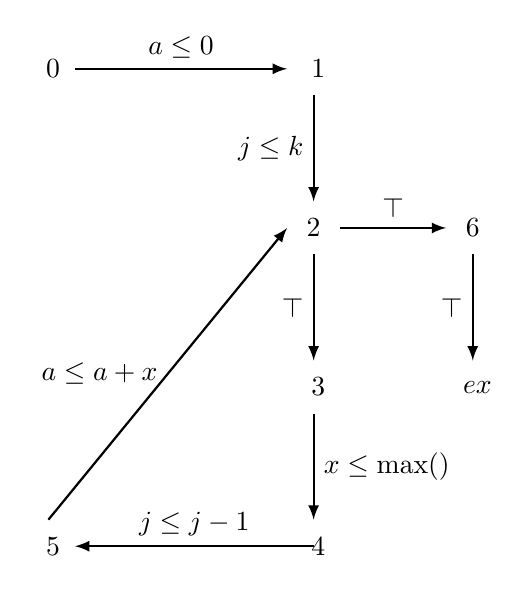
\begin{tikzpicture}[scale=\textwidth/18cm,samples=200]
\draw[] (-5, 10) circle (0pt) node{{ $0$}};
\draw[] (0, 10) circle (0pt) node{{ $1$}};
\draw[] (0, 7) circle (0pt) node{\textbf{$2$}};
\draw[] (0, 4) circle (0pt) node{{ $3$}};
\draw[] (0, 1) circle (0pt) node{{ $4$}};
\draw[] (-5, 1) circle (0pt) node{{ $5$}};
% Counter Variables
\draw[] (3, 7) circle (0pt) node {\textbf{$6$}};
\draw[] (3, 4) circle (0pt) node {{ $ex$}};
%
% Control Flow Edges:
\draw[ thick, -latex] (-4.5, 10)  -- node [above] {$a \leq 0$}(-0.5, 10);
\draw[ thick, -latex] (0, 9.5)  -- node [left] {$j \leq k$} (0, 7.5) ;
\draw[ thick, -latex] (0, 6.5)  -- node [left] {$\top$}  (0, 4.5);
\draw[ thick, -latex] (0, 3.5)  -- node [right] {$x \leq \max(\dbdom)$} (0, 1.5) ;
\draw[ thick, -latex] (0, 1)  -- node [above] {$j \leq j - 1$} (-4.5, 1) ;
\draw[ thick, -latex] (-5, 1.5)  -- node [left] {$a \leq a + x$} (-0.5, 7)  ;
\draw[ thick, -latex] (0.5, 7)  -- node [above] {$\top$}  (2.5, 7);
\draw[ thick, -latex] (3, 6.5)  -- node [left] {$\top$} (3, 4.5) ;
\end{tikzpicture}
 \caption{}
   \end{centering}
   \end{subfigure}
   \begin{subfigure}{.5\textwidth}
   \begin{centering}
   \begin{tikzpicture}[scale=\textwidth/18cm,samples=200]
\draw[] (0, 10) circle (0pt) node
{{ $a^0: {}^1_{0}$}};
\draw[] (0, 7) circle (0pt) node
{\textbf{$x^3: {}^{k}_{1}$}};
\draw[] (0, 4) circle (0pt) node
{{ $a^5: {}^{k}_{0}$}};
\draw[] (0, 1) circle (0pt) node
{{ $l^6: {}^{1}_{1}$}};
% Counter Variables
\draw[] (5, 9) circle (0pt) node {\textbf{$j^2: {}^{1}_{0}$}};
\draw[] (5, 6) circle (0pt) node {{ $j^4: {}^{k}_{0}$}};
%
% Value Dependency Edges:
\draw[ ultra thick, -latex, densely dotted,] (0, 1.5)  -- (0, 3.5) ;
\draw[ ultra thick, -latex, densely dotted,] (0, 4.5)  -- (0, 6.5) ;
\draw[ thick, -latex] (0, 7.5)  -- (0, 9.5) ;
\draw[ thick, -Straight Barb] (1.5, 3.5) arc (120:-200:1);
\draw[ thick, -Straight Barb] (6.5, 6.5) arc (150:-150:1);
\draw[ thick, -latex] (5, 6.5)  -- (5, 8.5) ;
% Control Dependency
\draw[ thick,-latex] (1.5, 7)  -- (4, 9) ;
\draw[ thick,-latex] (1.5, 4)  -- (4, 9) ;
\draw[ thick,-latex] (1.5, 7)  -- (4, 6) ;
\draw[ thick,-latex] (1.5, 4)  -- (4, 6) ;
\end{tikzpicture}
\caption{}
   \end{centering}
   \end{subfigure}
    \vspace{-0.3cm}
    \caption{(a) Example of data-flow analysis results for two rounds of adaptivity (b) The  weighted data-dependency graph from static analysis result.}
    \vspace{-0.5cm}
    \label{fig:dcfgraph_tworound}
\end{figure}
%

